\documentclass[a4paper]{article}
\usepackage[utf8]{inputenc}
\usepackage[spanish, es-tabla, es-noshorthands]{babel}
\usepackage[table,xcdraw]{xcolor}
\usepackage[a4paper, footnotesep = 1cm, width=20cm, top=2.5cm, height=25cm, textwidth=18cm, textheight=25cm]{geometry}
%\geometry{showframe}

\usepackage{tikz}
\usepackage{amsmath}
\usepackage{amsfonts}
\usepackage{amssymb}
\usepackage{float}
\usepackage{graphicx}
\usepackage{caption}
\usepackage{subcaption}
\usepackage{multicol}
\usepackage{multirow}
\setlength{\doublerulesep}{\arrayrulewidth}
\usepackage{booktabs}

\usepackage{hyperref}
\hypersetup{
    colorlinks=true,
    linkcolor=blue,
    filecolor=magenta,      
    urlcolor=blue,
    citecolor=blue,    
}

\newcommand{\quotes}[1]{``#1''}
\usepackage{array}
\newcolumntype{C}[1]{>{\centering\let\newline\\\arraybackslash\hspace{0pt}}m{#1}}
\usepackage[american]{circuitikz}
\usetikzlibrary{calc}
\usepackage{fancyhdr}
\usepackage{units} 

\graphicspath{{../Ejercicio-1/}{../Ejercicio-2/}{../Ejercicio-3/}{../Ejercicio-4/}}

\pagestyle{fancy}
\fancyhf{}
\lhead{22.01 Teoría de Circuitos}
\rhead{Mechoulam, Lambertucci, Rodriguez Turco, Londero, Galdeman}
\rfoot{\centering \thepage}

\begin{document}

\subsection{Celda universal}
Una celda universal es un conjunto de filtros RC activos de segundo orden, compuestos por amplificadores en cascada. Estos pueden estar dispuestos en diversas configuraciones, como lo son la sumadora, restadora, integradora, amplificadora o atenuadora. Estos filtros son también conocidos como celdas de variables de estado, debido al uso de dicho método para la resolución de las ecuaciones diferenciales. Las universales se caracteriza por poseer bajas sensibilidades con respecto a sus componentes, alta flexibilidad y buen rendimiento. Existen distintos tipos de configuraciones, donde cada una de estas posee sus respectivas ventajas y desventajas. A continuación, se procede a analizar cada una de ellas\footnote{L. Huelsman, Active and passive analog filter design, 2nd ed. New York: McGraw-Hill, 1993.}.

\subsubsection{Kerwin-Huelsman-Newcomb (KHN)}
La celda Kerwin-Huelsman-Newcomb %, nombre otorgado a partir de sus creadores\footnote{W. J. Kerwin, L. P. Huelsman, and R. W. Newcomb, ``State-Variable Synthesis for Insensitive Integrated Circuit Transfer Functions,'' \textit{IEEE Journal of Solid-State Circuits}, vol. 2, no. 3, pp. 87–92, Sep. 1967.},
puede ser comprendida con mayor facilidad a partir de un ejemplo. Se considera una transferencia de un filtro pasa banda:
\begin{equation}
	\frac{V_o(s)}{V_i(s)} = \frac{Ks}{s^2 + a_1 s + a_0}
\end{equation}

Se divide, tanto el numerador como el denominador de la expresión de la izquierda, por $s^2$.
\begin{equation}
	\frac{V_o(s)}{V_i(s)} = \frac{\frac{K}{s}}{1 + \frac{a_1}{s} + \frac{a_0}{s^2}}
	\label{equ:1}
\end{equation}

Se define
\begin{equation}
	V_a(s) = \frac{V_i(s)}{1 + \frac{a_1}{s} + \frac{a_0}{s^2}}
	\label{equ:2}
\end{equation}

Reescribinedo (\ref{equ:1}) con (\ref{equ:2}), se obtiene
\begin{equation}
	V_o(s) = \frac{K}{s} \cdot V_a(s)
	\label{equ:3}
\end{equation}

Si se utiliza la transformada de Laplace inversa tanto en (\ref{equ:2}) como en (\ref{equ:3}), se observa que se posee el siguiente sistema de ecuacuiones:
\begin{equation}
\begin{split}
	v_a(t) =\ v_i(t) - a_1 & \int v_a(t)dt - a_0 \int \left( \int v_a(t)dt \right) dt \\
	v_o(t) =& \ K\int \left( \int v_a(t)dt \right) dt
\end{split}
\end{equation}

De las ecuaciones anteriores, $v_a(t) = \ddot{x}(t) $, $\int v_a(t)dt = \dot{x}(t)$ y $\int \left( \int v_a(t)dt \right) dt = x(t)$ son las llamadas variables de estado. Dichas expresiones se pueden representar estas de la forma mostrada en la Figura (\ref{fig:blockKHN}).
\begin{figure}[H]
\centering
	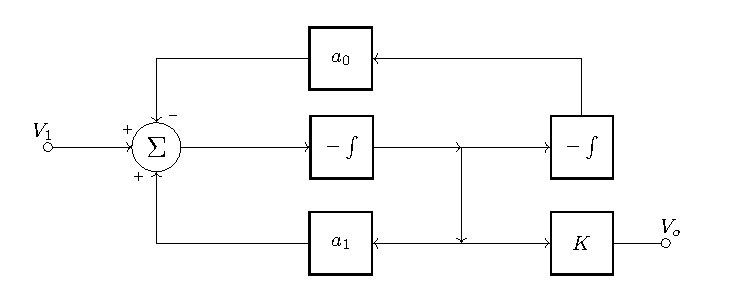
\includegraphics[width=0.7\textwidth]{ImagenesEjercicio4/Bloques-KHN.pdf}
	\caption{Diagrama de bloques de la celda KHN.}
	\label{fig:blockKHN}
\end{figure}

Es así que, para cada integrador se obtiene $V_{o3} = \frac{-V_{o2}}{sR_2C_2}$ y
$V_{o2} = \frac{-V_{o1}}{sR_1C_1}$, mientras que para el sumador
\begin{equation*}
	V_{o1} = -\frac{R_6}{R_5} V_{o3} + \frac{R_4}{R_3 + R_4} \frac{R_5 + R_6}{R_5} V_1 + \frac{R_3}{R_3 + R_4} \frac{R_5 + R_6}{R_5} V_{o2}
\end{equation*}

Finalmente, con las definiciones previas se puede elaborar el circuito presentado a continuación.
\begin{figure}[H]
\centering
	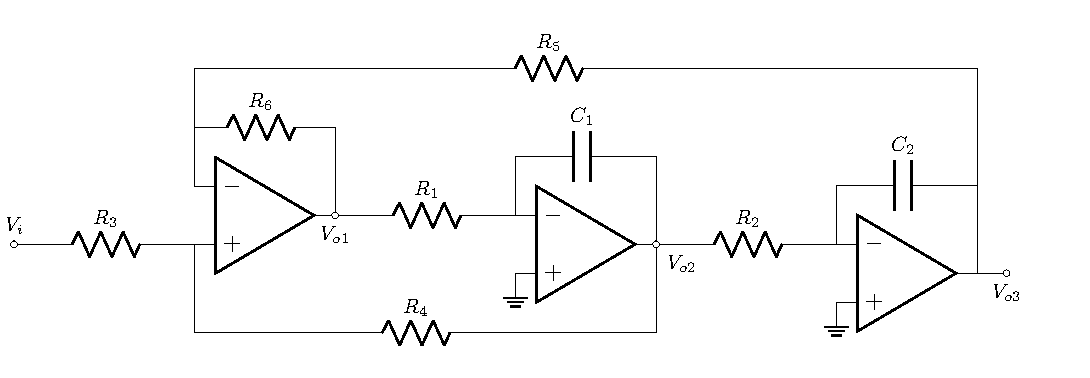
\includegraphics[width=0.9\textwidth]{ImagenesEjercicio4/KHN.pdf}
	\caption{Celda KHN.}
	\label{fig:KHN}
\end{figure}

Con todo lo establecido previamente se consigue determinar las siguientes transferencias:
\begin{equation}
	\frac{V_{o3}}{V_{i}} = \frac{R_5 + R_6}{R_4 + R_3} \frac{R_3}{R_5} \frac{1}{D(s)}
	\label{equ:pbajo}
\end{equation}

\begin{equation}
	\frac{V_{o2}}{V_{i}} = -\frac{R_5 + R_6}{R_4 + R_3} \frac{R_3}{R_5} \frac{s}{R_1 C_1 D(s)}
	\label{equ:pband}
\end{equation}

\begin{equation}
	\frac{V_{o1}}{V_{i}} = \frac{R_5 + R_6}{R_4 + R_3} \frac{R_3}{R_5} \frac{s^2}{D(s)}
	\label{equ:palto}
\end{equation}

Siendo
\begin{equation}
	D(s) = s^2 + \frac{s}{R_1 C_1} \frac{R_5 + R_6}{R_4 + R_3} \frac{R_3}{R_5} + \frac{R_6}{R_1 R_2 R_5 C_1 C_2}
\end{equation}

Observando (\ref{equ:pbajo}), (\ref{equ:pband}) y (\ref{equ:palto}), se denota que, tomando cada una de dichas salidas, esta celda puede ser utilizada como un pasa bajos, de banda pasante y pasa altos respectivamente. Es por ello que a partir de ahora se considera $V_{PA} = V_{o1}$, $V_{BP} = V_{o2}$ y $V_{PB} = V_{o3}$. Tanto la frecuencia de corte, como el factor Q de cada etapa, es el mismo, ya que comparten denominador, siendo estos
\begin{equation}
\begin{split}
	\omega_o = \sqrt{\frac{R_6}{R_1 R_2 R_5 C_1 C_2}} \\
	Q = \frac{R_3 + R_4}{R_5 + R_6} \frac{R_5}{R_3} \sqrt{\frac{R_1 R_6 C_1}{R_2 R_5 C_2}} 
\end{split}
\end{equation}

Es destacable la independencia que posee $\omega_o$ de $R_3$ y $R_4$ y la dependencia del factor $Q$ de dichas variables. Por lo tanto, es posible modificar esta ultima sin modificar la frecuencia de corte. Además, el termino $K$ previamente establecido, varía para cada salida. $K_{PB}$ representa la ganancia en continua para el pasa bajos, $K_{BP}$ la ganancia en la frecuencia de resonancia del pasa banda, y para el pasa altos, $K_{PA}$ es la ganancia en frecuencia infinita.
\begin{equation}
\begin{split}
	K_{PB} = \frac{R_5 + R_6}{R_3 + R_4} \frac{R_4}{R_6}	\	\	\ con \ \omega = 0 \\
	K_{BP} = -\frac{R_4}{R_3}	\	\	\ con \ \omega = \omega_o \\
	K_{PA} = \frac{R_5 + R_6}{R_3 + R_4} \frac{R_4}{R_5}	\	\	\ con \ \omega = \infty	
\end{split}
\end{equation}

Este tipo de celda, que cuenta con una entrada ($V_i$) y varias salidas ($V_{PB}$, $V_{BP}$ y $V_{PA}$), se la conoce como un sistema SIMO, debido a sus siglas del ingles ``single-in multi-out''. Se destaca también que la etapa que cumple el rol de pasa banda es inversora, mientras que las etapas de pasa bajos y altos no. Por otro lado, en caso de ser deseado que esta celda funcione como un rechaza banda o pasa todo, se debe agregar un cuarto amplificador operacional que actúe como restador de las tres señales previamente mencionadas para el caso del pasa todo, o entre las etapas pasa bajos y altos, para obtener el rechaza bandas\footnote{A. Sedra and K. Smith, Microelectronic Circuits, 5th ed. New York: Oxford University Press, 1991.}.
\begin{figure}[H]
\begin{center}
\begin{circuitikz}
	\node [circ](central){};
	\draw (central) -- ++(0,1) to[R, l=$R_{PA}$] ++(-2,0) node[ocirc, label=left:$V_{o1}$](){};
	\draw (central) to[R, l=$R_{BP}$] ++(-2,0) node[ocirc, label=left:$V_{o2}$](){};
	\draw (central) -- ++(0,-1) to[R, l=$R_{PB}$] ++(-2,0) node[ocirc, label=left:$V_{o3}$](){};
	\draw (central) -- ++(1,0) node[op amp, anchor=-](Amp){};
	\draw (Amp.+) node[ground](){};
	\draw (Amp.-) -- ++(0,1) to[R, l=$R_f$] ++(2.25,0) -| (Amp.out);
	\draw (Amp.out) -- ++(0.5,0) node[ocirc, label=right:$V_{f}$](){};
\end{circuitikz}
	\caption{Configuración restadora para obtener un rechaza banda con filtro KHN.}
	\label{fig:khninv}
\end{center}
\end{figure}

\subsubsection{Tow-Thomas (TT)}
La celda Tow-Thomas %, nombre dado por sus creadores\footnote{J. Tow, ``Design formulas for active RC filters using operational-amplifier biquad,'' \textit{Electronics Letters}, vol. 5, no. 15, pp. 339–341, Jul. 1969.}\footnote{L. C. Thomas, ``The Biquad: Part I-Some practical design considerations,'' \textit{IEEE Transactions on Circuit Theory}, vol. 18, no. 3, pp. 350–357, 1971.},
surge como una variación de la celda KHN. A esta última, se la modifica buscando aprovechar una realimentación negativa a base de una implementación RC. De esta forma, se logra alejar las frecuencias naturales del eje $j\omega$ por sobre el semiplano izquierdo. De igual forma que se realizó con la celda KHN, se construye el siguiente diagrama de bloques.
\begin{figure}[H]
\centering
	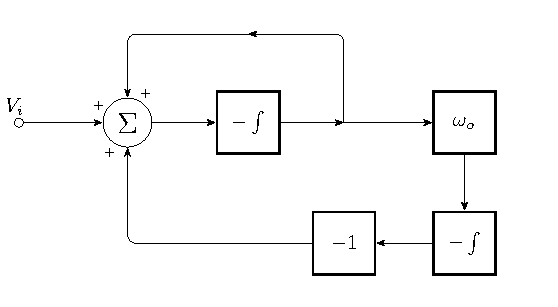
\includegraphics[width=0.7\textwidth]{ImagenesEjercicio4/Bloques-TT.pdf}
	\caption{Diagrama de bloques de la celda TT.}
	\label{fig:blockTT}
\end{figure}

Desarrollando en un circuito, se obtiene lo presentado en la Figura (\ref{fig:TT}).
\begin{figure}[H]
\centering
	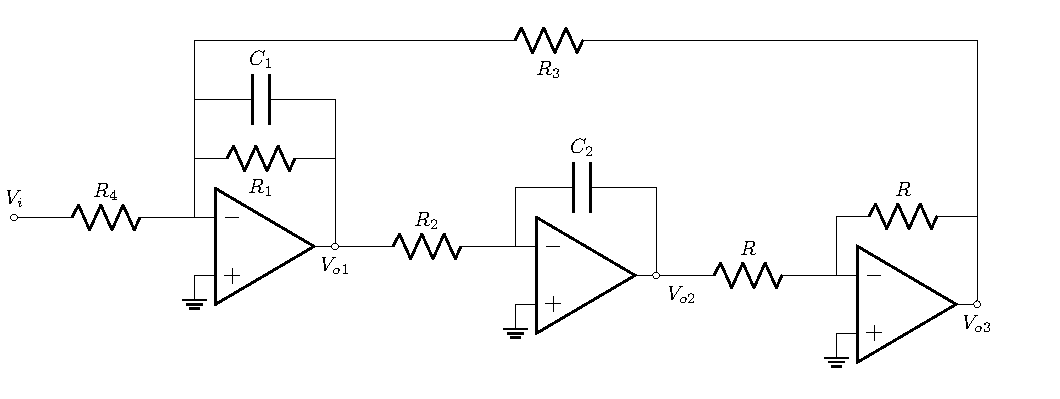
\includegraphics[width=0.9\textwidth]{ImagenesEjercicio4/TT.pdf}
	\caption{Celda TT.}
	\label{fig:TT}
\end{figure}

Analizando la tensión a la salida de cada operacional, se obtiene
\begin{equation}
	\frac{V_{o1}}{V_i} = -\frac{s}{R_4C_1}\frac{1}{D(s)}
\end{equation}
\begin{equation}
	\frac{V_{o2}}{V_i} = \frac{1}{R_2 R_4 C_1 C_2}\frac{1}{D(s)}
\end{equation}
\begin{equation}
	\frac{V_{o3}}{V_i} = -\frac{V_{o2}}{V_i}
\end{equation}

Siendo
\begin{equation}
	D(s) = s^2 + \frac{s}{R_1 C_1} + \frac{1}{R_2 R_3 C_1 C_2}
	\label{equ:dtt}
\end{equation}

De de la misma forma que con la celda KHN, de (\ref{equ:dtt}) se obtiene
\begin{equation}
\begin{split}
	\omega_o = \sqrt{\frac{1}{R_2 R_3 C_1 C_2}} \\
	Q = R_1 \sqrt{\frac{C_1}{R_2 R_3 C_2}} 
\end{split}
\end{equation}

De manera similar, se destaca el hecho de que la frecuencia $\omega_o$ es independiente de $R_1$, lo que permite modificar el factor $Q$ sin afectar a la otra variable. Se expresan ademas los valores de $K$ para cada caso.
\begin{equation}
\begin{split}
	K_{PB} = \frac{R3}{R_4}	\	\	\ con \ \omega = 0 \\
	|K_{BP}| = \frac{R_1}{R_4}	\	\	\ con \ \omega = \omega_o
\end{split}
\end{equation}

Se denota además que $V_{BP} = V_{o1}$ y $V_{PB} = V_{o2}$. Es así que la celda TT permite obtener un filtro pasa bandas y dos pasa bajos, siendo uno de ellos inversor. Este circuito no posee una transferencia que cumpla la función de pasa altos, por lo tanto, tampoco posee directamente una función de rechaza banda o pasa todo, al igual que la celda KHN.

\subsubsection{\r{A}ckerberg-Mossberg (AM)}
La celda \r{A}ckerberg-Mossberg resulta de una variación de la TT. Del circuito mostrado en la Figura (\ref{fig:TT}), se invierte el amplificador operacional utilizado para retroalimentar el sistema.
\begin{figure}[H]
\centering
	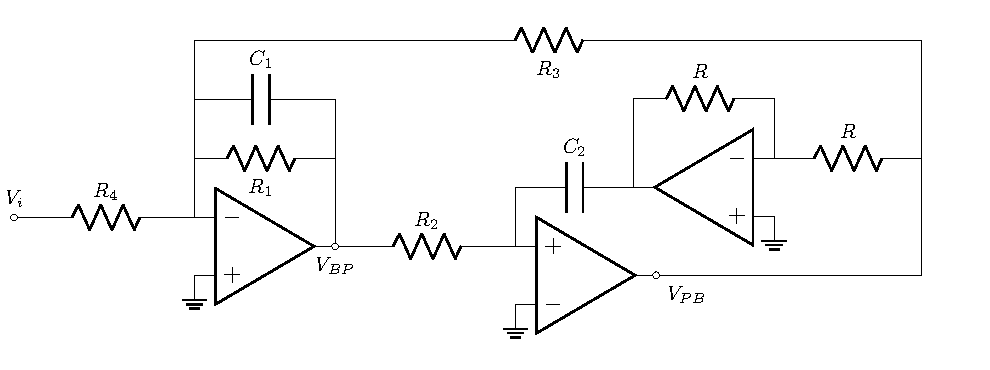
\includegraphics[width=0.9\textwidth]{ImagenesEjercicio4/AM.pdf}
	\caption{Celda AM.}
	\label{fig:AM}
\end{figure}

En consecuencia, este sistema posee las mismas características que el anterior, poseyendo también las mismas transferencias y sensibilidades. Cabe destacar que esta configuración posee mejor compensación de fase a altas frecuencias.

\subsubsection{Fleischer-Tow (FT)}
En ocasiones es deseable poseer una señal de entrada que alimente varios nodos, obteniendo una única salida. Así como se denotó la existencia de sistemas SIMO, el caso previamente mencionado cae dentro de la definición lo que se conoce como sistemas MISO, suyas siglas en ingles significan ``multi-in single-out''. A continuación se presenta la celda Fleischer-Tow, la cual se caracteriza por poder presentar una única transferencia que, dependiendo de los componentes seleccionados, puede ser un pasa bajaso, pasa altos, pasa todo, de banda pasante y rechaza banda\footnote{R. Raut and M. N. S. Swamy, Modern Analog Filter Analysis and Design, 1st. ed. Weinheim: John Wiley and Sons, 2010.}.
\begin{figure}[H]
\centering
	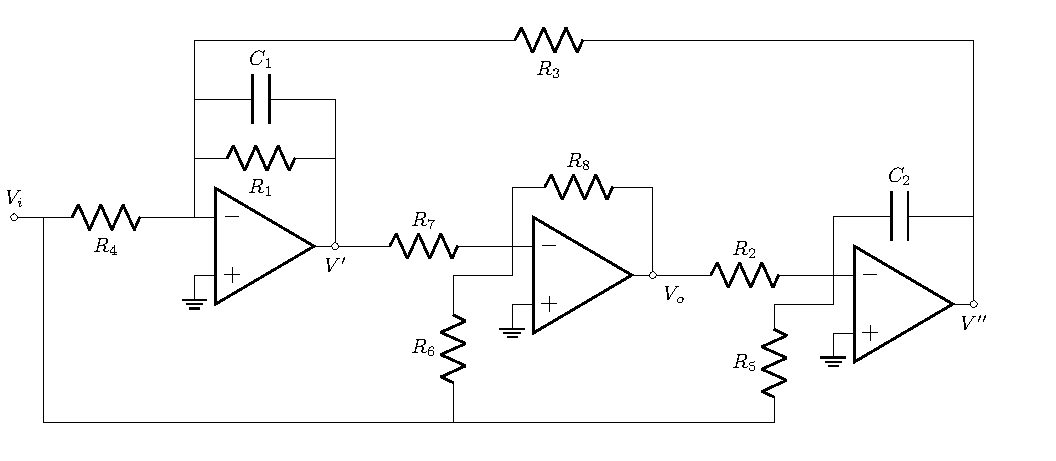
\includegraphics[width=0.9\textwidth]{ImagenesEjercicio4/FT.pdf}
	\caption{Celda FT.}
	\label{fig:FT}
\end{figure}

%\begin{table}[H]
%\centering
%\begin{tabular}{ccc}
%\hline
%\textbf{Tipo de filtro} & \textbf{Componentes} & \textbf{Observaciones} \\
%\hline
%Pasa Bajos & $R_4=R_6=\infty$, $R_5=\frac{R}{|K_{PB}|}$ & $K_{PB} = H(0) < 0$ \\
%Banda Pasante & $R_5=R_6=\infty$, $R_4=\frac{R Q}{K_{BP}}$ & $K_{BP} = H(\omega_o) > 0$ \\
%Pasa Altos & $R_5=\infty$, $R_4 = \frac{R Q}{|K_{PA}|}$, $R_6=\frac{R'}{|K_{PA}|}$ & $K_{PA} = H(\infty) < 0$ \\
%Rechaza Banda & $R_5=\frac{\omega_{o}^{2} R}{\omega_{\infty}^{2} |K_{RB}|}$, $R_4 = \frac{R Q}{|K_{RB}|}$, $R_6=\frac{R'}{|K_{RB}|}$ & $K_{RB} = H(\infty) < 0$ \\ %, $\omega_{\infty}$ frecuencia de notch \\
%Pasa Todo & $R_5=\frac{R}{|K_{PT}|}$, $R_4 = \frac{R Q}{2 |K_{PT}|}$, $R_6=\frac{R'}{|K_{PT}|}$ & $K_{PT} = H(\omega) < 0$ \\
%\hline
%\end{tabular}
%\caption{Tipos de filtro y componentes para una celda FT.}
%\label{tabla:tiposdefiltroft}
%\end{table}

Se decide obtener la función transferencia de esta celda, en un principio, considerando los operacionales ideales, por cuestiones que explicadas más adelante. Para calcular la función mencionada de esta celda, se observa primero la siguiente configuración:
\begin{figure}[H]
\centering
\begin{circuitikz}
	\node [ocirc, label=left:$V_a$](va){};
	\draw (va.east) to[generic, l=$Z_1$] ++(3,0) node[op amp, anchor=-](A1){};
	\draw (va) ++(0.5,0) node[](v1aux1){};
	\draw (A1.+) node[ground](){};
	\draw (A1.out) node[](aux1){};	
	\draw (A1.-) -- ++(0,1) to[generic, l=$Z_3$] ++(2.25,0) -| (aux1.center);
	\draw (A1.out) -- ++(0.5,0) node[ocirc, label=below:$V_c$](){};
	\draw (A1.-) -- ($ (A1.-) !.7! (A1.+) $) to[generic, l=$Z_2$] ++(-3,0) node[ocirc, label=left:$V_b$](vb){};
\end{circuitikz}
\caption{Circuito genérico inversor.}
\label{fig:generic}
\end{figure}

Observando la Figura (\ref{fig:generic}), aplicando el teorema de superposición, se obtiene que
\begin{equation}
	V_c = -\frac{V_a}{\frac{Z_1}{Z_3} + \frac{Z_1}{Z_3 A_o} + \frac{1}{A_o}} - \frac{V_b}{\frac{Z_2}{Z_3} + \frac{Z_2}{Z_3 A_o} + \frac{1}{A_o}}
	\label{equ:generic}
\end{equation}

Aplicando (\ref{equ:generic}) y considerando los tres operacionales de la Figura (\ref{fig:FT}) iguales, se obtiene el siguiente sistema de ecuaciones:
\begin{equation}
\begin{split}
	V' = - V_i A - V'' B \\
	V_o = - V' C - V_i D \\
	V'' = - V_o E - V_i F
\end{split}
\end{equation}
siendo las constantes empleadas las siguientes:
\begin{equation}
\begin{split}
	A^{-1} =& \ \frac{R_4}{R_1 // \frac{1}{sC_1}} + \frac{R_4}{\left( R_1 // \frac{1}{sC_1} \right) A_o} + \frac{1}{A_o} \\
	B^{-1} =& \ \frac{R_3}{R_1 // \frac{1}{sC_1}} + \frac{R_3}{\left( R_1 // \frac{1}{sC_1} \right) A_o} + \frac{1}{A_o} \\
	C^{-1} =& \ \frac{R_7}{R_8} + \frac{R_7}{R_8 A_o} + \frac{1}{A_o} \\
	D^{-1} =& \ \frac{R_6}{R_8} + \frac{R_6}{R_8 A_o} + \frac{1}{A_o} \\
	E^{-1} =& \ sC_2R_2 + \frac{sC_2R_2}{A_o} + \frac{1}{A_o} \\
	F^{-1} =& \ sC_2R_5 + \frac{sC_2R_5}{A_o} + \frac{1}{A_o}
\end{split}
\end{equation}

Operando algebraicamente, se obtiene que la transferencia de esta configuración es
\begin{equation}
	\frac{V_o}{V_i} = \frac{AC - BCF - D}{1 + BCE}
	\label{equ:transf-ft-r}
\end{equation}

Si se consideran ideales los operacionales, es decir, se toma $A_o \rightarrow \infty$, se obtiene que la forma de la transferencia final es
\begin{equation}
	\frac{V_o}{V_i} = - \frac{R_2}{R_5} \frac{s^{2} \frac{C_1 C_2 R_3 R_5 R_7}{R_6} + s \frac{C_2 R_3 R_5 R_7}{R_1} \left( \frac{1}{R_6} - \frac{R_1}{R_4 R_7} \right) + 1}{s^{2} \frac{C_1 C_2 R_2 R_3 R_7}{R_8} + s \frac{C_2 R_2 R_3 R_7}{R_1 R_8} + 1}
\label{equ:transf-ft-i}
\end{equation}

De esta última ecuación se puede obtener los siguientes valores de interés.
\begin{equation}
\begin{split}
	\omega_o = \sqrt{\frac{R_8}{R_2 R_3 R_7 C_1 C_2}} \\
	Q = R_1 \sqrt{\frac{C_1 R_8}{C_2 R_2 R_3 R_7}} 
\end{split}
\label{equ:woq-ft}
\end{equation}

Es así que se destaca la dependencia de $\omega_o$ y $Q$ de los capacitores, mientras que resultan ser independientes de $R_5$. Finalmente, y el detalle más importante, es que, a diferencia de, por ejemplo, las celdas KHN y TT, no hay componente que modifique una variable y no la otra. Por lo tanto, una modificación de uno de estos factores, genera un cambio en el otro.

\subsection{Filtro a desarrollar}
Una vez presentado cada tipo de celda, solo resta determinar cual conviene emplear para realizar el filtro con las características deseadas.

Se busca confeccionar un filtro con las siguientes características:
\begin{table}[H]
\centering
\begin{tabular}{cc}
\hline
\textbf{Variable} & \textbf{Valor} \\
\hline
$f_\infty$ & $30 \ kHz$ \\
$\Delta f_a$ & $600 \ Hz$ \\
$\Delta f_p$ & $13.2 \ kHz$ \\
$A_a$ & $40 \ dB$ \\
$A_p$ & $6 \ dB$ \\
$Z_{in}(f)$ & $50 \ k\Omega$ \\
Filtro & Rechaza Banda \\
Plantilla & Chebycheff Inverso \\
\hline
\end{tabular}
\caption{Características del filtro a realizar.}
\label{tabla:caracteristicas1}
\end{table}

Como se busca confeccionar un filtro rechaza banda, se descartan los filtros TT y AM, ya que estos no poseen transferencias que sean pasa altos, por lo tanto no se puede confeccionar directamente un filtro del tipo notch. De forma similar, si bien la celda KHN posee transferencia pasa altos, se requiere un amplificador operacional extra que permita restar la pasa bajos y pasa altos, por lo cual también queda descartada. Por último para la celda FT basta con tomar los componentes adecuados, consiguiendo así la transferencia deseada. Es por ello que la celda considerada más optima para este caso es la FT. Esta es la razón por la cuál en (\ref{equ:generic}) se optó por considerar los operacionales reales.

Con lo establecido en la Tabla (\ref{tabla:caracteristicas1}), y sabiendo que se debe cumplir
\begin{equation}
\begin{split}
	f_{\infty}^{2} = f_{p}^{-} f_{p}^{+} = f_{a}^{-} & f_{a}^{+} \\
	\Delta f_p = f_{p}^{+} - f_{p}^{-} \\
	\Delta f_a = f_{a}^{+} - f_{a}^{-} 
\end{split}
\end{equation}
se calculan las frecuencias de cada banda:
\begin{table}[H]
\centering
\begin{tabular}{cc}
\hline
\textbf{Variable} & \textbf{Valor} \\
\hline
$f_{p}^{-}$ & $30984 \ Hz$ \\
$f_{a}^{-}$ & $36701 \ Hz$ \\
$f_{a}^{+}$ & $37301 \ Hz$ \\
$f_{p}^{+}$ & $44184\ Hz$ \\
\hline
\end{tabular}
\caption{Características del filtro a realizar.}
\label{tabla:caracteristicas2}
\end{table}

\begin{center}
	\Large{\textbf{\textcolor{red}{CUENTAS DE PLANTILLA. \\ JUSTIFICACIÓN DE n, Q y COMPONENTES.}}}
\end{center}

\subsubsection{Análisis de sensibilidades}
\begin{center}
	\Large{\textbf{\textcolor{red}{CUENTAS: LEER CONSIGNA PARA VER QUE SENSIBILIDADES PIDE.}}}
\end{center}

\subsubsection{Confección del filtro y mediciones}

Respetando lo presentado en la Figura (\ref{fig:FT}), considerando lo observado en (\ref{equ:transf-ft-i}) y en (\ref{equ:woq-ft}) y considerando que el filtro es de orden 2, se seleccionaron los componentes presentados en la Tabla (\ref{tab:componentes}). Se destaca que, para ambos casos, se seleccionó $R_4 = R_5 = R_6 = 47 \ k\Omega$ y $C_1 = C_2 = 10 \ nF$.

\begin{table}[H]
\centering
\begin{tabular}{ccccccccc}
\hline 
 & $R_1$ & $R_2$ & $R_3$ & $R_7$ & $R_8$ & $Q_Z$ & $Q_P$ & $f_o$ \\
 \hline
$1^{er}$ Etapa & 1547 $\Omega$ & 46.38 k$\Omega$ & 121.22 $\Omega$ & 1547 $\Omega$ & 34.2 k$\Omega$ & $\infty$ & 3.07 & 31.56 kHz \\
$2^{da}$ Etapa & 1.2 k$\Omega$ & 55.2 k$\Omega$ & 150 $\Omega$ & 1.2 k$\Omega$ & 64.35 k$\Omega$ & $\infty$ & 3.05 & 40.50 kHz \\
\hline
\end{tabular}
\caption{Componentes seleccionados.}
\label{tab:componentes}
\end{table} 

Se decidió colocar en lugar de los capacitores pines hembra, los cuales permiten reemplazar con facilidad dichos componentes. Esto se debe a que los que se disponen son de una tolerancia del $10 \%$. De esta forma, se vale del analizador de impedancias para determinar la capacitancia de estos y así garantizar el uso del capacitor adecuado. Por otro lado, como la impedancia de entrada resulta del paralelo entre las resistencias $R_4$, $R_5$ y $R_6$, lo cual implica $Z_{in} = 15.67 \ k\Omega$, se coloca un buffer a la entrada de cada instancia, ya que de esta forma, la impedancia de entrada del circuito es la del buffer, garantizando que ambas instancias se acoplen adecuadamente. 
Al momento de realizar las placas, se optó por colocar jumpers, de forma tal que se pueda hacer las mediciones deseadas con y sin dichos buffers, para poder realizar comparaciones.   

Es así que se presentan a continuación las mediciones realizadas.
%\begin{figure}[H]
%\centering
%	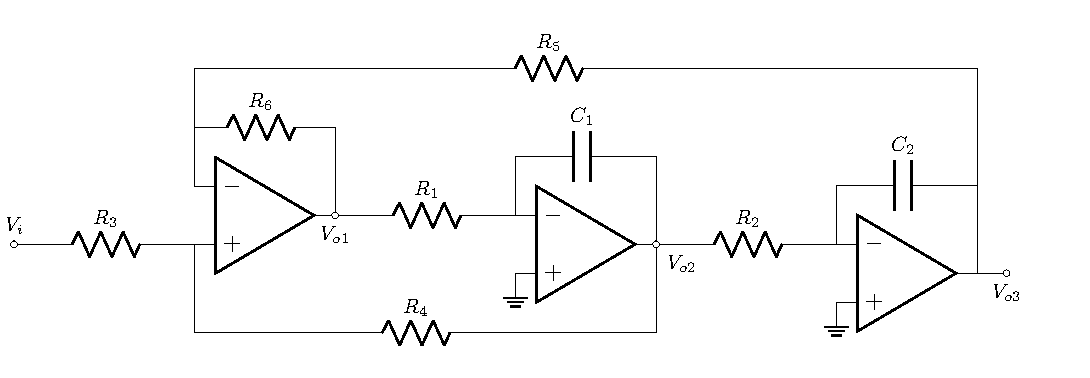
\includegraphics[width=0.9\textwidth]{ImagenesEjercicio4/KHN.pdf}
%	\caption{Celda KHN.}
%	\label{fig:KHN}
%\end{figure}

\end{document}